\documentclass{article}

\usepackage[final]{style}
\usepackage[utf8]{inputenc}
\usepackage[brazilian]{babel}
\usepackage[T1]{fontenc}
\usepackage{hyperref}
\usepackage{url}
\usepackage{booktabs}
\usepackage{amsfonts}
\usepackage{microtype}
\usepackage{xcolor}
\usepackage{graphicx}
\graphicspath{{../output/}}
\usepackage{listings}
\usepackage{multicol}
\usepackage{amsmath}
\usepackage[font=footnotesize]{caption}
\DeclareMathOperator*{\argmin}{arg\!min}
\usepackage{subcaption}
\definecolor{blue}{RGB}{41,5,195}
\makeatletter
\hypersetup{colorlinks=true,linkcolor=blue,citecolor=red,urlcolor=blue}
\makeatother

\renewcommand{\figureautorefname}{Figura}
\newcommand{\media}[1]{\ensuremath{\bar{#1\vphantom{+1}}}}

\title{Relatório\\Segunda Lista de Exercícios}

\author{
  Rodrigo Ferreira Berriel\\
  LCAD @ UFES
}


\begin{document}

\maketitle

\begin{abstract}
  Esse relatório visa apresentar os resultados alcançados com a segunda lista de exercícios, bem como responder as questões feitas em cada exercício. Além desse relatório, foi enviado o código-fonte para a reprodução dos resultados apresentados nesse relatório. O código-fonte também se encontra disponível no GitHub:
  
  \url{http://github.com/rodrigoberriel/aprendizado-de-maquina-2017-1}
\end{abstract}

\section{Exercício 1}

Para a base \texttt{Car Evaluation} (disponível em \url{http://archive.ics.uci.edu/ml/}), considerando que o primeiro atributo é $x_1$, o segundo é $x_2$ e assim por diante, estime as probabilidades:

\paragraph{a)} $P(x_1=\text{med})$ e $P(x_2=\text{low})$

\begin{itemize}
	\item $P(x_1=\text{med}) = 25.00\%$
	\item $P(x_2=\text{low}) = 25.00\%$
\end{itemize}

\paragraph{b)} $P(x_6=\text{high} | x_3=2)$ e $P(x_2=\text{low} | x4=4)$

\begin{itemize}
	\item $P(x_6=\text{high} | x_3=2) = 33.33\%$
	\item $P(x_2=\text{low} | x4=4) = 25.00\%$
\end{itemize}

\paragraph{c)} $P(x_1=\text{low}|x_2=low,x_5=\text{small})$ e $P(x_4=4|x_1=\text{med},x_3=2)$

\begin{itemize}
	\item $P(x_1=\text{low}|x_2=low,x_5=\text{small}) = 25.00\%$
	\item $P(x_4=4|x_1=\text{med},x_3=2) = 33.33\%$
\end{itemize}

\paragraph{d)} $P(x_2= \text{vhigh},x_3=2|x_4=2)$ e $P(x_3=4,x_5=\text{med}|x_1=\text{med})$

\begin{itemize}
	\item $P(x_2= \text{vhigh},x_3=2|x_4=2) = 6.25\%$
	\item $P(x_3=4,x_5=\text{med}|x_1=\text{med}) = 8.33\%$
\end{itemize}

\section{Exercício 2}

Aplique o Naive Bayes sobre a base de dados \texttt{Balance Scale} (disponível em \url{http://archive.ics.uci.edu/ml/}) utilizando o procedimento de Hold-Out dez vezes, na proporção de 75\% de amostras de treino e 25\% de teste. Obtenha a acurácia média e o desvio padrão da acurácia. Realize os experimentos:

\paragraph{a)} Considerando uma distribuição Gaussiana dos atributos;

\begin{itemize}
	\item Acurácia: $91.03\%$
	\item Desvio Padrão: $2.09\%$
\end{itemize}

\paragraph{b)} Discretizando os valores (em 5 partes cada atributo);

\begin{itemize}
	\item Acurácia: $91.73\%$
	\item Desvio Padrão: $1.75\%$
\end{itemize}

\paragraph{c)} Discretize os valore da mesma forma que em b) usando a suavização de Laplace.

\begin{itemize}
	\item Acurácia: $91.73\%$
	\item Desvio Padrão: $1.75\%$
\end{itemize}

Os valores sem e com a suavização de Laplace foram iguais por causa da \textit{seed} usada em todos os experimentos. Testando com outras \textit{seeds}, percebe-se uma variação.

\section{Exercício 3}

Para a rede bayesiana da figura abaixo (ver figura na lista de exercícios original), verifique as seguintes afirmações, indicando se é falso ou verdadeiro e fornecendo a devida explicação.

\paragraph{a)} A é independente de C
\begin{itemize}
	\item Verdadeiro, pois D e seus descendentes não são conhecidos, i.e., não foram observados.
\end{itemize}

\paragraph{b)} A é independente de C tal que foi observado D
\begin{itemize}
	\item Falso, pois D bloqueia o caminho entre A e C, quando observado.
\end{itemize}

\paragraph{c)} A é independente de C tal que foi observado H
\begin{itemize}
	\item Falso, pois como H é descendente de D, a mesma lógica da \textit{b)} pode ser aplicada.
\end{itemize}

\paragraph{d)} F é independente de C
\begin{itemize}
	\item Falso, pois há uma conexão serial (C $\rightarrow$ D $\rightarrow$ F) e D não é conhecido.
\end{itemize}

\paragraph{e)} G é independente de C tal que foi observado I
\begin{itemize}
	\item Verdadeiro, pois I (conexão serial) foi observado, bloqueando o caminho entre C e G; e J (conexão convergente) não foi observado.
\end{itemize}

\paragraph{f)} G é independente de C tal que foram observados I e J
\begin{itemize}
	\item Falso, pois a observação de J (C $\rightarrow$ J $\leftarrow$ G) causa dependência entre C e G.
\end{itemize}

\paragraph{g)} I é independente de A tal que foi observado E
\begin{itemize}
	\item Falso, pois E, (um descendente de D), foi observado, causando a dependência entre I e A.
\end{itemize}

\paragraph{h)} E e F são independentes de B tal que foi observado D
\begin{itemize}
	\item Verdadeiro, pois D, quando observado, bloqueia os caminhos para E e F a partir de B.
\end{itemize}

\section{Exercício 4}

Dois observadores em lugares distintos obtêm medidas diferentes $M_1$ e $M_2$ do número de estrelas $N$ em uma pequena região do céu, usando telescópios. Cada telescópio pode (com uma pequena probabilidade $f$) estar fora de foco (eventos $F_1$ e $F_2$), e nesse caso o astrônomo deixará de contar 3 estrelas ou mais (se $N$ for menor ou igual a 3 ele não contará nenhuma estrela).

\paragraph{a)} Quais das redes abaixo (ver figuras na lista original) são representações corretas da informação acima?

As redes \textit{ii)} e \textit{iii)}. A rede \textit{i)} está incorreta, pois caso as medidas $M_1$ e $M_2$ sejam conhecidas, essa rede diz que $N$ é independente dos focos ($F_1$ e $F_2$), o que não é verdade.

\paragraph{b)} Qual é a melhor rede? Explique.

Dado que ambas as redes estão corretas, a rede \textit{ii)} pode ser considerada melhor, pois necessita de menos parâmetros.

\section{Exercício 5}

Para a base \texttt{Car Evaluation} (disponível em \url{http://archive.ics.uci.edu/ml/}):

\paragraph{a)} Construa uma árvore de decisão com dois níveis de nó de decisão (isto é, o primeiro nó de decisão (primeiro nível), os nós de decisão abaixo dele (segundo nível) e em seguida os nós folha) usando a medida de Ganho de Informação. Selecione aleatoriamente 75\% dos dados para treinamento que serão usados para construir a árvore. Retorne a estrutura da árvore construída.

Os dados da base foram pré-processados de tal forma que as variáveis categóricas foram convertidas para uma escala numérica. Isso foi possível, pois as categorias apresentam uma ordem lógica. A estrutura da árvore de decisão pode ser vista na \autoref{fig:exercicio5-a}.

\begin{figure}[h]
	\centering
	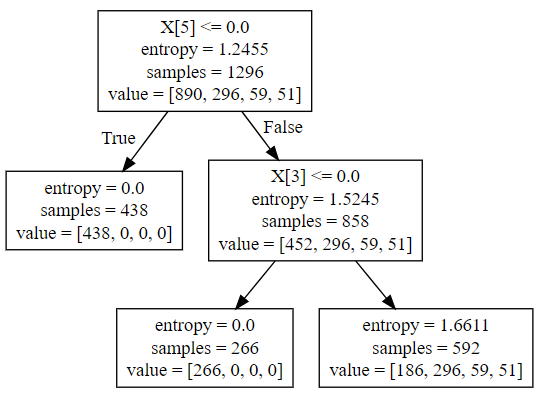
\includegraphics[width=0.5\linewidth]{exercicio5-a.png}
	\caption{Estrutura da Árvore de Decisão, construída usando a medida de Ganho de Informação.}
	\label{fig:exercicio5-a}
\end{figure}

\paragraph{b)} Use os restantes 25\% dos dados para avaliação. Retorne a acurácia obtida.

Avaliando nos 25\% restantes dos dados, a árvore de decisão alcança uma acurácia de 79.63\%.

\paragraph{c)} Tente obter as regras de decisão a partir da árvore construída.

Revertendo os valores para suas respectivas categorias, podemos obter as seguintes regras:

\begin{itemize}
	\item R1: $x_5 = \text{low} \rightarrow \text{unacc}$
	\item R2: $x_5 \neq \text{low}, x_3 = 2 \rightarrow \text{unacc}$
	\item R3: $x_5 \neq \text{low}, x_3 \neq 2 \rightarrow \text{acc}$
\end{itemize}

\section{Exercício 6}

Para a base \texttt{Servo} (disponível em \url{http://archive.ics.uci.edu/ml/}):

\paragraph{a)} Construa uma árvore de regressão com dois níveis de nó de decisão (isto é, o primeiro nó de decisão (primeiro nível), os nós de decisão abaixo dele (segundo nível) e em seguida os nós folha) usando a medida de redução de desvio padrão. Selecione aleatoriamente 75\% dos dados para treinamento que serão usados para construir a árvore. Retorne a estrutura da árvore construída.

A estrutura da árvore de regressão pode ser vista na \autoref{fig:exercicio6-a}.

\begin{figure}[h]
	\centering
	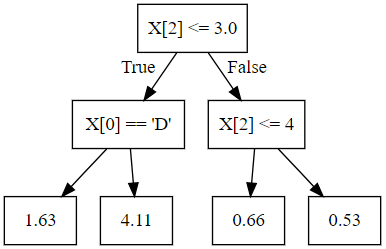
\includegraphics[width=0.5\linewidth]{exercicio6-a.png}
	\caption{Estrutura da Árvore de Regressão, construída usando a medida de Redução do Desvio Padrão.}
	\label{fig:exercicio6-a}
\end{figure}

\paragraph{b)} Use os restantes 25\% dos dados para avaliação. Retorne as medidas MAPE e RMSE.

Avaliando nos 25\% restantes dos dados, a árvore de regressão alcança:

\begin{itemize}
	\item RMSE: $1.30$
	\item MAPE: $72.74\%$
\end{itemize}

\paragraph{c)} Tente obter as regras de decisão a partir da árvore construída.

A partir da \autoref{fig:exercicio6-a}, podemos obter as seguintes regras de decisão:

\begin{itemize}
	\item R1: $x_2 \leq 3, x_0 = \text{D} \rightarrow 1.63$
	\item R2: $x_2 \leq 3, x_0 \neq \text{D} \rightarrow 4.11$
	\item R3: $x_2 > 3, x_2 \leq 4 \rightarrow 0.66$
	\item R4: $x_2 > 3, x_2 > 4 \rightarrow 0.53$
\end{itemize}

\section{Exercício 7}

Para as bases de dados \texttt{Spiral} e \texttt{Jain} (disponíveis em \url{http://cs.joensuu.fi/sipu/datasets/}), agrupe os dados em 3 e 2 grupos, respectivamente, usando kmeans e clusterização hierárquica. Avalie os resultados com a métrica de pureza, que é calculada de forma semelhante a acurácia: para cada cluster verifique qual foi a classe predominante, amostras pertencentes a outras classes estão no grupo errado. O resultado da métrica é o número total de amostras predominantes nos clusters dividido pelo número total de amostras, multiplicado por 100\%. Calcule também a métrica distância intra-inter clusters, mostrada abaixo (ver na lista original). Faça os experimentos com a distância Euclidiana. Gere gráficos com os grupos formados pelo kmeans e clusterização hierárquica. Comente os resultados e os métodos usados. Lembre-se de não usar o atributo da classe para agrupar os dados.

As fórmulas para a dist\_intra\_inter podem ser vistas na lista original.

O algoritmo kMeans foi aplicado nas bases de dados propostas e os resultados alcançados foram:

\begin{itemize}
	\item Spiral (\autoref{fig:exercicio7-kmeans-spiral})
	\begin{itemize}
		\item Pureza: 34.62\%
		\item Dist\_intra\_inter: 73.81\%
	\end{itemize}
	\item Jain (\autoref{fig:exercicio7-kmeans-jain})
	\begin{itemize}
		\item Pureza: 78.55\%
		\item Dist\_intra\_inter: 72.35\%
	\end{itemize}
\end{itemize}

Os gráficos para o kMeans podem ser vistos na \autoref{fig:exercicio7-kmeans}.

\begin{figure*}[h!]
	\centering
	\begin{subfigure}[t]{0.49\textwidth}
		\centering
		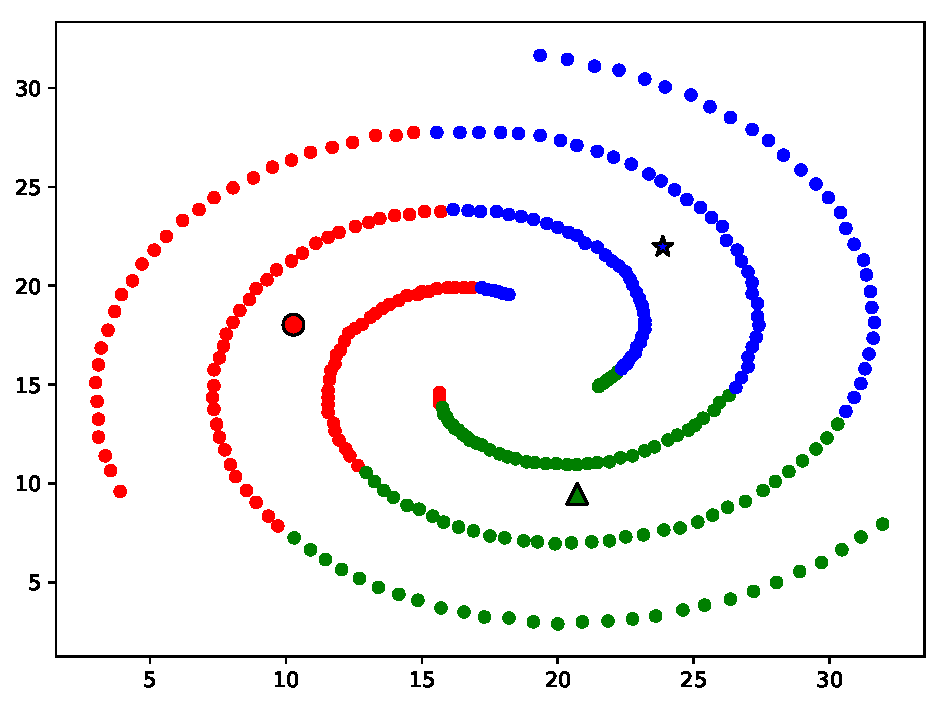
\includegraphics[width=\linewidth]{exercicio7-kmeans-spiral.pdf}
		\caption{kMeans aplicado no Spiral}
		\label{fig:exercicio7-kmeans-spiral}
	\end{subfigure}%
	~ 
	\begin{subfigure}[t]{0.49\textwidth}
		\centering
		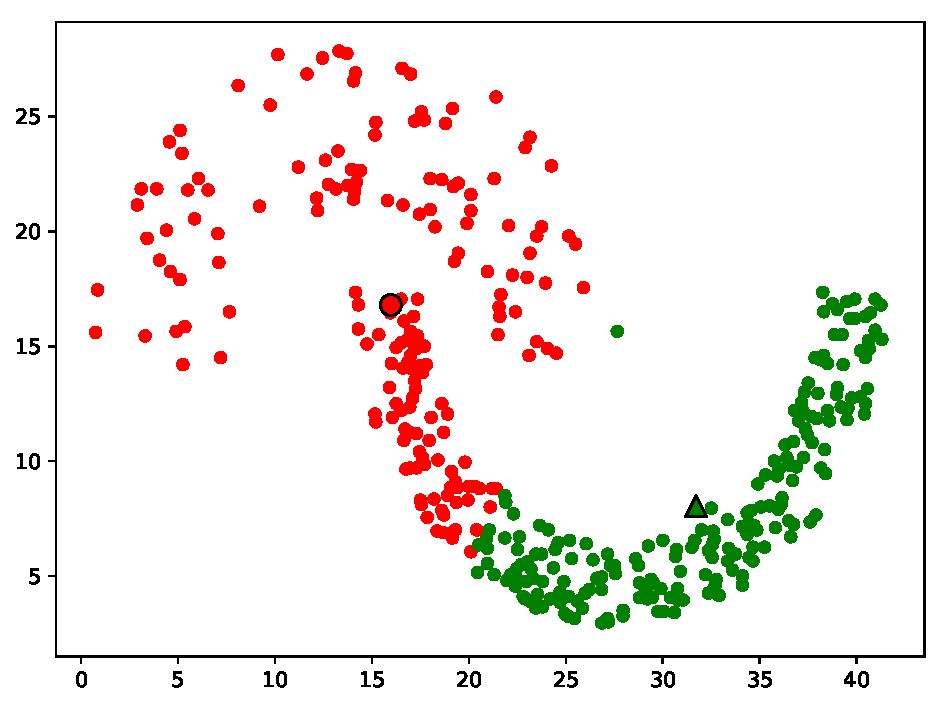
\includegraphics[width=\linewidth]{exercicio7-kmeans-jain.pdf}
		\caption{kMeans aplicado no Jain}
		\label{fig:exercicio7-kmeans-jain}
	\end{subfigure}
	\caption{Algoritmo kMeans aplicado nas bases de dados Spiral e Jain.}
	\label{fig:exercicio7-kmeans}
\end{figure*}

O algoritmo AGNES (Agglomerative Nesting) foi aplicado nas bases de dados propostas e os resultados alcançados foram:

\begin{itemize}
	\item Spiral (\autoref{fig:exercicio7-agnes-spiral})
	\begin{itemize}
		\item Pureza: 100.00\%
		\item Dist\_intra\_inter: 444.73\%
	\end{itemize}
	\item Jain (\autoref{fig:exercicio7-agnes-jain})
	\begin{itemize}
		\item Pureza: 80.97\%
		\item Dist\_intra\_inter: 87.07\%
	\end{itemize}
\end{itemize}

Os gráficos para o AGNES podem ser vistos na \autoref{fig:exercicio7-kmeans}.

\begin{figure*}[h!]
	\centering
	\begin{subfigure}[t]{0.49\textwidth}
		\centering
		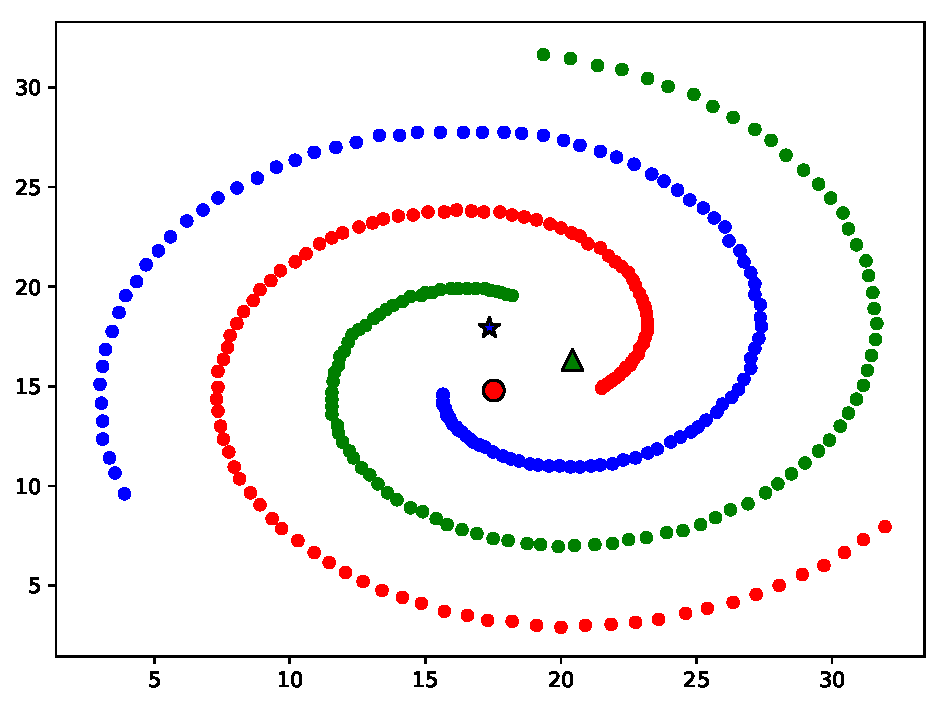
\includegraphics[width=\linewidth]{exercicio7-agnes-spiral.pdf}
		\caption{AGNES aplicado no Spiral}
		\label{fig:exercicio7-agnes-spiral}
	\end{subfigure}%
	~ 
	\begin{subfigure}[t]{0.49\textwidth}
		\centering
		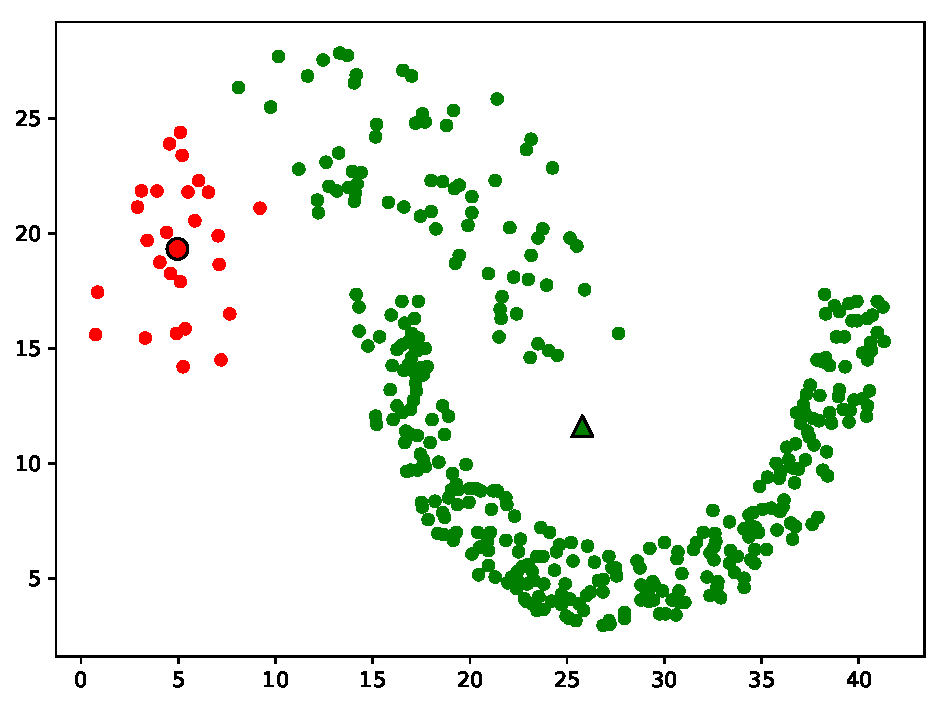
\includegraphics[width=\linewidth]{exercicio7-agnes-jain.pdf}
		\caption{AGNES aplicado no Jain}
		\label{fig:exercicio7-agnes-jain}
	\end{subfigure}
	\label{fig:exercicio7-agnes}
	\caption{Algoritmo AGNES (Agglomerative Nesting) aplicado nas bases de dados Spiral e Jain.}
\end{figure*}

Os resultados acima demonstram que as bases de dados favorecem algoritmos de clusterização hierárquica. O AGNES, usando a conexão com o mais próximo (Slide 67 da Aula 8), alcança altos índices de pureza nas duas bases de dados, incluindo pureza máxima na base de dados Spiral. A vantagem do kMeans fica na tempo de execução\footnote{A implementação de ambos foi ingênua, havendo espaço para otimização em ambos os casos.}, conseguindo convergir rapidamente (14 e 11 iterações para a base de dados Spiral e Jain, respectivamente). É interessante observar que, para a base de dados Spiral, a métrica dist\_intra\_inter fica maior conforme a pureza tende a 100\%.


\section*{Instruções para usar os scripts}

O código-fonte enviado foi desenvolvido em Python. Esse código foi testado tanto no Linux (Ubuntu 14.04) quanto no Windows 10. Para rodar os scripts dos exercícios, é necessário ter Python 2.7 ou Python 3.x instalado na sua máquina e algumas dependências. Para instalar as dependências, basta rodar o comando abaixo na raiz do repositório:

\begin{verbatim}
	$ pip install -r lista2/requirements.txt
\end{verbatim}

Para executar o script de um exercicio em específico (por exemplo, o exercício 1), basta executar:

\begin{verbatim}
	$ cd lista2/scripts
	$ python lista2.py --exercicio=1
\end{verbatim}

Ou então, se preferir, você pode executar o script diretamente. Por exemplo:

\begin{verbatim}
	$ cd lista2/scripts
	$ python exercicio1.py
\end{verbatim}

As bases de dados Car Evaluation, Balance Scale, Spiral, Jain e Servo serão baixadas automaticamente nas questões em que foram usadas. Todas as bases de dados estão armazenadas na pasta \texttt{data}. Ao executar os scripts, os gráficos que estão neste relatório serão exibidos e salvos na pasta \texttt{output}. O codigo-fonte desse relatório (em \LaTeX) também se encontra na pasta \texttt{report}. Para garantir a reprodutibilidade dos resultados e gráficos, foi usado como seed o valor \texttt{2017} definido no arquivo \texttt{scripts/constants.py}.

\end{document}
